\section{Continual Post-Training and Model Merging}

\begin{frame}{}
    \LARGE Alignment and Post-Training: \textbf{Continual Post-Training and Merging}

    \vspace{1em}
    \normalsize A deployed model is never finished. How do you add to it without breaking what it knew?
\end{frame}

\begin{frame}{A 2026 Map of Continual Learning}
    \begin{itemize}\itemsep0.4em
        \item A 2026 survey sorts continual learning for LLMs along three axes:
    \end{itemize}
    \begin{center}
    \small
    \renewcommand{\arraystretch}{1.3}
    \begin{adjustbox}{max width=\linewidth}\begin{tabular}{l>{\raggedright\arraybackslash}p{7.6cm}}
        \toprule
        \textbf{When} & pre-training, post-training, inference time \\
        \textbf{How} & off-policy, on-policy, beyond gradients \\
        \textbf{Where} & parameters, or memory, skills and protocols \\
        \bottomrule
    \end{tabular}\end{adjustbox}
    \end{center}
    \vspace{0.4em}
    \begin{itemize}\itemsep0.4em
        \item The survey's thesis: adaptation is moving from the \textbf{parameters} to the \textbf{system} around them.
        \item This section stays with the parameters: continued pre-training, fine-tuning, RL and merging.
    \end{itemize}
    \src{Hou et al., ``Continual Learning in Transition,'' \href{https://arxiv.org/abs/2608.06216}{arXiv:2608.06216} (abstract).}
\end{frame}

\begin{frame}{Domain Adaptation: What It Buys and What It Costs}
    \begin{center}
    \small
    \begin{adjustbox}{max width=\linewidth}\begin{tabular}{l>{\raggedright\arraybackslash}p{3.5cm}>{\raggedright\arraybackslash}p{3.4cm}>{\raggedright\arraybackslash}p{3.1cm}}
        \toprule
        \textbf{Model} & \textbf{Continued on} & \textbf{Gain} & \textbf{Cost} \\
        \midrule
        Code Llama 34B & 85\% code, 8\% code-related text, 7\% general text & HumanEval 22.6 to 48.8\% & GSM8K falls 42.2 to 32.7 \\
        Llemma 34B & 95\% maths, 5\% replay & MATH 12.2 to 25.0, GSM8K 29.6 to 51.5 & 23K A100-hours (7B run) \\
        AdaptLLM 7B & raw biomedical or finance text & domain knowledge & prompting \alert{falls}: 44.2 to 41.7 \\
        \bottomrule
    \end{tabular}\end{adjustbox}
    \end{center}
    \begin{itemize}\small\itemsep0.2em
        \item A 7\% replay share protected language, but not every off-domain skill: Code Llama lost 9.5 points of maths.
        \item Raw domain text can teach facts and still damage the ability to \emph{answer questions}. AdaptLLM's fix: turn the documents into reading-comprehension tasks, mixed with general instructions.
        \item \textbf{Part of the forgetting is optimisation.} Re-warming the learning rate raises the loss even on the \emph{same} data. Replay of only 1\% already reduces forgetting.
    \end{itemize}
    \src{Rozi\`ere et al., ``Code Llama,'' \href{https://arxiv.org/abs/2308.12950}{arXiv:2308.12950}, Tables 1 and 12. Azerbayev et al., ``Llemma,'' \href{https://arxiv.org/abs/2310.10631}{arXiv:2310.10631}. Cheng, Huang, Wei, ``AdaptLLM,'' ICLR 2024, \href{https://arxiv.org/abs/2309.09530}{arXiv:2309.09530}. Ibrahim et al., \href{https://arxiv.org/abs/2403.08763v4}{arXiv:2403.08763v4}, Sections 6.2 and 7.1.}
\end{frame}

\begin{frame}{Fine-Tuning Forgets by Law}
    \begin{itemize}\itemsep0.4em
        \item \textbf{A scaling law for forgetting.} $\mathcal{L}_{ft}$ is the fine-tuning loss. $\mathcal{L}_f$ measures forgetting as the cross-entropy of the fine-tuned model against the base model's next-token predictions on held-out text (WikiText-103). $c$ and $s$ are fitted constants per fine-tuning dataset:
    \end{itemize}
    \[
        \mathcal{L}_{f}=-c\,\mathcal{L}_{ft}+s
    \]
    \begin{itemize}\itemsep0.4em
        \item Forgetting is \emph{linear} in the fine-tuning loss, with $R^2$ of 0.95 and 0.97 on two datasets. The more the fine-tune learns, the more it forgets.
        \item Neither early stopping nor a different LoRA rank escapes the line.
        \item For RL, LoRA matches full fine-tuning even at rank 1. Policy gradient absorbs only about $O(1)$ bits per episode.
    \end{itemize}
    \vspace{0.3em}
    \src{Kalajdzievski, ``Scaling Laws for Forgetting When Fine-Tuning Large Language Models,'' \href{https://arxiv.org/abs/2401.05605v1}{arXiv:2401.05605v1}, Sections 3.1 and 4.1, Eq. 4 and Figure 2. Schulman, ``LoRA Without Regret'' (Thinking Machines, 2025).}
\end{frame}

\begin{frame}{SFT or RL: Which Forgets Less?}
    \centering
    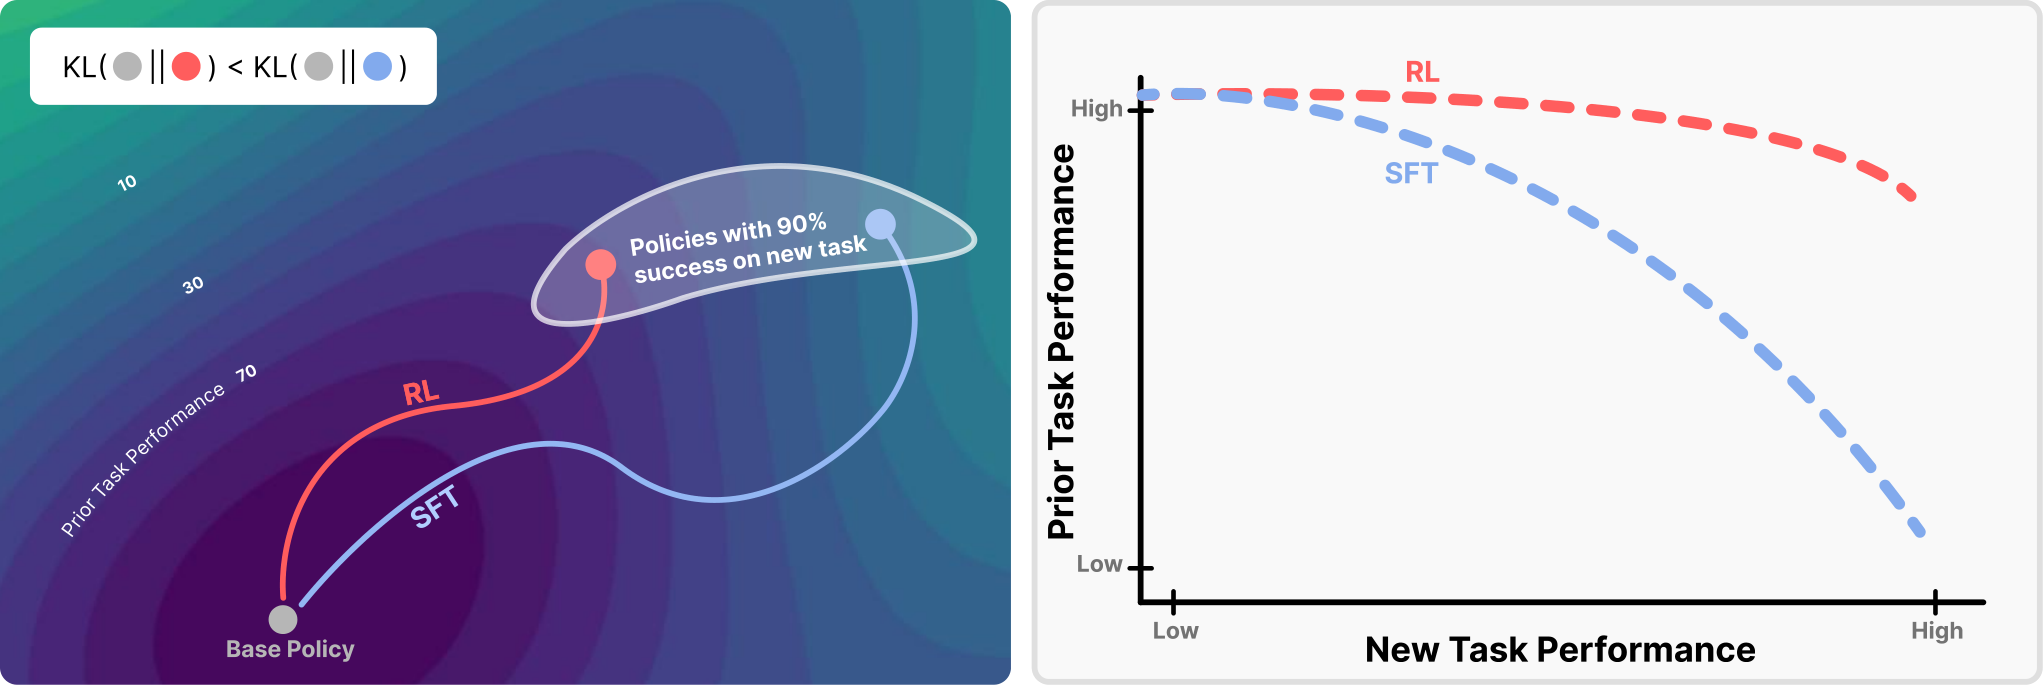
\includegraphics[width=0.74\linewidth,height=0.26\textheight,keepaspectratio]{images/alignment-post-training/rlrazor_fig1_teaser.png}
    \begin{columns}[T,onlytextwidth]
        \column{0.36\textwidth}
        \centering
        \small
        \begin{adjustbox}{max width=\linewidth}\begin{tabular}{lcc}
            \toprule
            \textbf{Llama-3.1-8B} & \textbf{Target} & \textbf{Other} \\
            \midrule
            SFT & $+25.2$ & $-27.8$ \\
            \rowcolor{KAUSTcyan!12} RL & $+18.4$ & $-3.4$ \\
            \bottomrule
        \end{tabular}\end{adjustbox}
        \column{0.62\textwidth}
        \begin{itemize}\itemsep0.3em
            \item \textbf{RL's Razor.} RL finds the solution closest in KL to the base model. Forgetting tracks $\mathbb{E}_{x}\big[\mathrm{KL}(\pi_0\,\|\,\pi)\big]$ on the \emph{new} task's inputs.
            \item \textbf{The debate.} A second study finds a weaker link to KL (correlation 0.52) and credits \emph{on-policy data} instead.
        \end{itemize}
    \end{columns}
    \vspace{0.2em}
    \caveat{This holds for a \textbf{single} new task. In sequential multi-task RL, the drift happens on old tasks and RL does forget (2026).}
    \src{Shenfeld, Pari, Agrawal, ``RL's Razor: Why Online RL Forgets Less,'' \href{https://arxiv.org/abs/2509.04259}{arXiv:2509.04259}, Figure 1. Chen et al., ``Retaining by Doing,'' \href{https://arxiv.org/abs/2510.18874}{arXiv:2510.18874}. Luo et al., ``RL Forgets! Towards Continual Policy Optimization,'' \href{https://arxiv.org/abs/2607.04364}{arXiv:2607.04364}.}
\end{frame}

\begin{frame}{Merging Inside Real Recipes}
    \begin{itemize}\itemsep0.3em
        \item \textbf{Against the alignment tax.} RLHF raises the reward while reading comprehension and translation scores fall. Interpolating back toward the base model gave the best trade-off among all methods compared, including replay, LoRA and a KL penalty:
    \end{itemize}
    \[
        \theta=(1-\alpha)\,\theta_0+\alpha\,\theta_{\text{RLHF}}, \qquad \alpha=0.2 \text{ by default}
    \]
    \begin{center}
    \small
    \begin{adjustbox}{max width=\linewidth}\begin{tabular}{l>{\raggedright\arraybackslash}p{10.8cm}}
        \toprule
        \textbf{Recipe} & \textbf{How merging is used} \\
        \midrule
        OLMo 2 & average several mid-training runs that differ only in data order \\
        T\"ulu 3 & linear averaging with mergekit \\
        SmolLM3 & merge the aligned model 0.9 to 0.1 with the mid-training checkpoint, to recover long-context performance at 128k \\
        \bottomrule
    \end{tabular}\end{adjustbox}
    \end{center}
    \begin{itemize}\itemsep0.3em
        \item \textbf{A 2026 limit.} For combining several RL specialists, multi-teacher on-policy distillation beat weight merging.
    \end{itemize}
    \src{Lin et al., ``Mitigating the Alignment Tax of RLHF,'' EMNLP 2024, \href{https://arxiv.org/abs/2309.06256}{arXiv:2309.06256}. OLMo 2, \href{https://arxiv.org/abs/2501.00656}{arXiv:2501.00656}. T\"ulu 3, \href{https://arxiv.org/abs/2411.15124}{arXiv:2411.15124}. Bakouch et al., ``SmolLM3'' (Hugging Face, 2025). MOPD, \href{https://arxiv.org/abs/2606.30406}{arXiv:2606.30406}.}
\end{frame}

\begin{frame}{Lifelong Adaptation in Deployed Systems}
    \begin{center}
    \small
    \begin{adjustbox}{max width=\linewidth}\begin{tabular}{>{\raggedright\arraybackslash}p{3.3cm}>{\raggedright\arraybackslash}p{5.3cm}>{\raggedright\arraybackslash}p{4.7cm}}
        \toprule
        \textbf{System} & \textbf{What is updated, and when} & \textbf{Evidence} \\
        \midrule
        \rowcolor{KAUSTcyan!12} Cursor Tab (production) & policy gradient on live user data, a new checkpoint every 1.5 to 2 hours & 21\% fewer suggestions, 28\% higher accept rate \\
        SEAL & the model writes its own fine-tuning data, rewarded by RL if the update helps & no-context question answering: 32.7 to 47.0\% \\
        \bottomrule
    \end{tabular}\end{adjustbox}
    \end{center}
    \begin{itemize}\itemsep0.4em
        \item \textbf{Reward design as product design.} Cursor pays $+0.75$ for an accepted suggestion, $-0.25$ for a rejected one, 0 for silence. The policy then speaks only when $P(\text{accept})>25\%$.
    \end{itemize}
    \src{Cursor, ``Improving Cursor Tab with online RL'' (2025). Zweiger et al., ``Self-Adapting Language Models,'' \href{https://arxiv.org/abs/2506.10943}{arXiv:2506.10943}.}
\end{frame}

\begin{frame}{Continual Post-Training: What to Remember}
    \begin{itemize}\itemsep0.6em
        \item Part of the forgetting in continued pre-training is \textbf{optimisation}: re-warming the learning rate raises the loss even on the same data. Even 1\% replay helps.
        \item Domain adaptation has a bill. Check \textbf{off-domain skills} and \textbf{prompting ability}, not only the target benchmark.
        \item Forgetting is \textbf{linear} in the fine-tuning loss. Early stopping and a different LoRA rank stay on the same line.
        \item On-policy updates forget less for a single task. Sequential RL still forgets.
        \item Merging is now a routine pipeline step: against the alignment tax, across data orders, and to recover a lost skill.
    \end{itemize}
    \vspace{0.3em}
    \takeaway{\textbf{Next.} We have every component. The last section assembles them into one pipeline, using the recipes whose code and data are fully public.}
\end{frame}
